\chapter{Solution proposée}
\renewcommand{\leftmark}{\thechapter.~~Solution proposée}
Dans le chapitre précédent, les différentes solutions existantes pour faire
du CCMP ont été analysées. La solution jugée la plus efficace
est Remote Clip, celle-ci proposant une architecture P2P adéquate et un
niveau de sécurité correct. Pour ces raisons, certaines idées mises en avant
par Remote Clip seront réutilisées. De même des messages seront envoyés en
broadcast afin d'auto-configurer le réseau comme fait dans The Network
Clipboard.

\section{Principes d'une architecture P2P}\label{sec:p2p}
Avant de décrire l'architecture qui sera utilisée, il est préférable
de rappeler quels sont les principes de base d'une architecture P2P.
Habituellement, une architecture client-serveur est utilisée lorsqu'il
faut fournir un service à un ensemble de machines connectées en réseau,
c'est-à-dire que chaque client va se connecter à un (ou parfois plusieurs)
serveur central qui s'occupera de fournir le service désiré. Par opposition à
ce mode de fonctionnement centralisé, un réseau organisé en pair-à-pair
permet de se passer de serveur central, chaque client jouant à la fois le rôle
de client et de serveur. La figure \ref{fig:p2p} illustre la différence
de topologie réseau existante entre ces deux types d'architectures réseau.
De manière plus précise les systèmes P2P sont définis dans \cite{AS04} comme
étant:
\begin{quote}
  des systèmes distribués constitués de noeuds interconnectés, capables de
  s'auto-organiser dans des topologies de réseaux avec comme but le partage
  de ressources, telles que le contenu, les cycles CPU, le stockage,
  la bande passante tout en ayant la capacité de s'adapter aux erreurs et
  de s'accommoder de populations de noeuds transitoires; tout en maintenant
  une connectivité et des performances acceptables sans requérir
  l'intermédiaire ou le support d'un serveur ou d'une autorité
  centralisée globalement.
\end{quote}

Les difficultés potentielles à mettre en avant dans ce genre de systèmes
sont la gestion des va-et-vient de clients et la tolérance aux erreurs
sans l'aide de serveur central, et tout en minimisant la charge sur le réseau,
due à cette gestion. Il faut cependant noter que l'importance de la tolérance
aux erreurs est tout de même assez minime dans le contexte du copier/coller.
Les données stockées sont en général destinées à être utilisées à court terme
et non pas à être stockées de manière persistante. De même le nombre de pairs
est normalement peu élevé, et donc le nombre de va-et-vient n'est pas aussi
important que sur des systèmes à grande échelle.

Une remarque supplémentaire à faire est qu'une différence est souvent faite
entre réseaux P2P structurés et non structurés \cite{AS04, Lua05asurvey}.
Les premiers ont une topologie contrôlée de manière précise permettant
de placer chaque donnée à un endroit précis et d'effectuer des recherches
efficaces. Le réseau ici étant censé être de taille relativement petite
et le contenu changeant très rapidement, il n'est pas nécessaire de structurer
le réseau. En effet, le fait de structurer le réseau, en utilisant par exemple
une table de hashage distribuée, a comme intérêt d'avoir une complexité
algorithmique sous-linéaire en fonction du nombre de pairs présent dans
le réseau. Ici la taille du réseau étant fortement réduite, cette
complexité a peu d'impact sur les performances du logiciel. Le fait de ne
pas utiliser une table de hashage distribuée permet donc d'avoir un protocole
plus simple sans perte de performances.

\begin{figure}[!h]
  \centering
  % \input{fig_p2p.tex}
  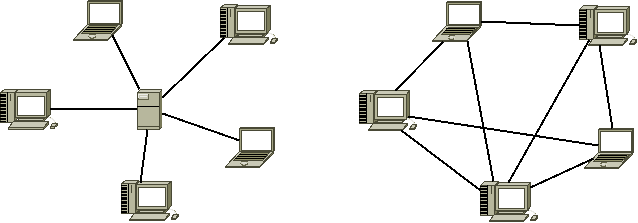
\includegraphics[width=\textwidth]{fig_p2p}
  \caption{Exemple de différence entre une topologie client-serveur et P2P}
  \label{fig:p2p}
\end{figure}

\section{Architecture logicielle}
Afin de suivre le principe \emph{KISS} (Keep It Simple Stupid, \emph{cf.}
Annexe \ref{ann:kiss}) et la philosophie Unix, le projet sera divisé en
plusieurs programmes, chacun d'entre eux s'occupant d'une tâche particulière.
Une autre raison justifiant une telle conception est le fait qu'elle introduit
la possibilité de développer le projet de manière incrémentale, en se
concentrant d'abord sur l'aspect réseau et ensuite sur l'implémentation
propre à un environnement particulier.

\subsection{Client P2P}
Premièrement un logiciel s'occupant uniquement de la gestion du presse-papier
sur le réseau est nécessaire. Celui-ci a comme rôle de se connecter aux
autres pairs et de s'organiser avec ceux-ci quand cela est nécessaire.
Sa seule fonctionnalité est en fait de gérer la partie réseau du système,
toute interaction locale (\emph{i.e.} avec l'utilisateur) se fait par
l'intermédiaire d'autres logiciels qui seront définis par la suite.

Il faut définir de manière plus précise comment l'ensemble des clients P2P
vont s'organiser afin de s'informer pour savoir quel client \emph{détient} le
presse-papier, comment un pair entre dans le réseau et comment détecter
qu'un pair a quitté celui-ci (volontairement ou pas).

\subsubsection{Gestion du presse-papier en P2P}
Il y a principalement deux possibilités pour gérer le presse-papier
sur le réseau. Lorsqu'un copier est effectué en local, le client P2P
doit prévenir les autres pairs qu'il détient le presse-papier.
La première option est d'envoyer en même temps la donnée copiée à tous les
pairs. La deuxième est de n'envoyer cette donnée que lorsque qu'un coller
est effectué chez un pair, celui-ci peut alors demander la donnée au pair
détenant le presse-papier.
La première manière de faire a les avantages et inconvénients suivants:
\begin{itemize}
\item Avantages:
  \begin{itemize}
  \item Possibilité de garder une copie du presse-papier sur chaque pair.
  \item Tolérance aux erreurs dans le cas où le pair détenant le presse-papier
    aurait quitté le réseau.
  \item Absence de communications réseaux en cas de multiples coller.
  \end{itemize}
\item Inconvénients:
  \begin{itemize}
  \item Consommation de bande passante accrue dans le cas où des copiers
    sont effectués fréquemment car il faudra envoyer la même donnée à chacun
    des pairs qui ne feront peut être pas forcément de coller. De plus la
    consommation de bande passante dépend du nombre de pair présent sur le
    réseau.
  \end{itemize}
\end{itemize}
La seconde a les avantages et inconvénients suivants:
\begin{itemize}
\item Avantages:
  \begin{itemize}
  \item Il n'est pas nécessaire de notifier l'ensemble des pairs à chaque
    copier: si un pair effectue plusieurs copies d'affilée, il ne faudrait
    notifier le réseau qu'une seule fois et sans envoyer la moindre donnée.
  \item En général le coller ne sera effectué que par un seul pair,
    il n'a donc qu'à demander lui même au pair détenant le presse-papier
    de la lui envoyer.
  \end{itemize}
\item Inconvénients:
  \begin{itemize}
  \item Faible tolérance aux erreurs: impossibilité de récupérer le
    presse-papier d'un pair ayant quitté le réseau.
  \item Si plusieurs collers ont lieu les uns à la suite des autres, il faudra
    demander plusieurs fois la même donnée au pair détenant le presse-papier.\\
  \end{itemize}
\end{itemize}

\subsubsection{X Window}
Avant de choisir entre une de ces deux solutions, il est important de
savoir ce qu'est X Window et comment ce logiciel fonctionne\cite{nye1992xlib}.
X est un standard pour les systèmes d'exploitations basés sur Unix permettant
d'afficher des éléments graphiques sur un écran plutôt qu'un terminal.
Il est principalement responsable de la couche la plus basse des systèmes
de fenêtrages de la majorité des systèmes Unix. Son fonctionnement est basé
sur une architecture client-serveur où X Window est le logiciel serveur
et chaque application graphique est un client. Lorsqu'un copier est réalisé au
sein d'une application, le client (\emph{i.e.} la fenêtre) notifie le serveur X
qu'un copier a eu lieu. le serveur retient alors que la dernière application
à avoir copié du texte est le client en question.

Lorsqu'une deuxième
application effectue un coller, elle demande d'abord au serveur quel client
a fait le dernier coller. Il peut ensuite demander à ce client de délivrer
le contenu de son presse-papier. Il faut noter que si le client responsable
du presse-papier a disparu, \emph{i.e.} si la fenêtre a été fermée, et qu'aucun
copier n'a été effectué depuis la fermeture du client, alors il est
impossible de récupérer la donnée et le presse-papier est considéré comme vide.
\footnote{Il faut cependant noter que si un logiciel d'historique de
presse-papier est utilisé, c'est le gestionnaire de presse-papier qui est
responsable de la donnée copiée. Il est donc normal si celle-ci est toujours
disponible après avoir fermé la fenêtre dans laquelle la donnée a été
initialement copiée.}
En fin de compte, il est clair que la description du fonctionnement de X Window
est la deuxième solution décrite précédemment.

\subsubsection{Choix d'une solution pour la gestion et
synchronisation du presse-papier}
Il faut donc faire un choix entre une de ces deux solutions. Un des critères
définit au début de ce travail étant de cibler Unix, il semble idéal de se
baser sur X Window pour implémenter une nouvelle solution. De même, Remote
Clip, ayant été décrit comme la meilleure solution rencontrée, fonctionne
de la même manière. Cependant en fin compte, c'est la première solution qui
est choisie. Celle-ci est plus intuitive et a surtout l'avantage d'être
tolérante aux erreurs. Et même si Remote Clip a été identifiée comme
solution idéale, un intérêt de réimplémenter une nouvelle solution est
d'améliorer ses fonctionnalités, en améliorant ici la tolérance aux erreurs.
Un dernier avantage qui sera discuté dans le chapitre \ref{chap:implem}
est le fait qu'envoyer la donnée à chaque pair à chaque copier facilite
la gestion d'historique synchornisé du presse-papier sans avoir à ajouter
cette fonctionnalité directement dans le logiciel nouvellement produit.

\subsubsection{Rejoindre le réseau}
Outre un moyen d'authentification, il est nécessaire de définir comment
un pair peut rejoindre le réseau afin de partager son presse-papier.
Une première solution consiste, pour un pair voulant
rejoindre le réseau, à connaître l'adresse IP et l'identifiant d'au moins un
autre pair déjà présent dans le réseau et connaissant les autres pairs présents
dans ce réseau. Il suffit alors de contacter cet autre pair et de synchroniser
la  liste des pairs de l'ensemble du réseau. Une autre solution envisageable
est d'utiliser un mécanisme de broadcast permettant de flooder le réseau pour
rechercher les pairs désirant rejoindre le réseau. Cette solution sera celle
utilisée, celle-ci permettant de minimiser le nombres de paramètres que devra
configurer l'utilisateur.

Pour cela, il faut que chaque pair envoie à interval régulier un message
en broadcast, sur le réseau local, permettant d'identifier le groupe de pairs
auquel il appartient ou veut appartenir. Tout pair appartenant au groupe et
recevant le message doit alors contacter le pair ayant envoyé le message en
ouvrant une connexion TCP. Il faut cependant faire attention à un
problème: le nombre de connexions TCP ouvertes peut devenir une charge
importante pour le réseau. En effet pour un groupe de $n$ pair, $n-1$
connexions sera ouverte pour chaque pair. Le nombre de connexions serait donc
en $O(n^2)$. Cependant le réseau P2P étant limité à quelques pairs dans le
cas du CCMP, ceci n'est pas handicapant.

De même afin d'ouvrir plusieurs fois une connexion TCP avec un pair déjà
connu, il faut gérer une table des pairs dans laquelle sera ajouté un
pair identifié. Les figures \ref{fig:broadcast} et \ref{fig:connections}
illustrent par des diagrammes d'états comment un pair se comporte pour
contacter les autres pairs du réseaux.

\begin{figure}[!h]
  \centering
  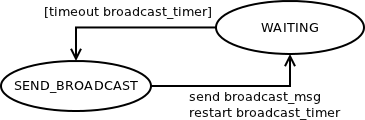
\includegraphics{broadcast}
  \caption{Diagramme d'états modélisant l'envoi de messages en broadcast
    par le client P2P.}
  \label{fig:broadcast}
\end{figure}

\begin{figure}[!h]
  \centering
  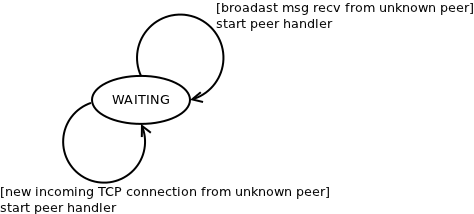
\includegraphics[width=\textwidth]{connections}
  \caption{Diagramme d'états modélisant le comportement du client P2P lors
    de la réception d'un message broadcast et lors de l'acceptation d'une
    connexion TCP.}
  \label{fig:connections}
\end{figure}

\subsubsection{Quitter le réseau}
Lorsqu'un pair quitte le réseau, il doit notifier l'ensemble des autres
pairs de son départ. Une fois ceci fait, il peut fermer chaque connexion
ouverte avec chacun des pairs. En revanche il se peut qu'un pair quitte
le réseau sans pouvoir notifier les pairs de son départ, \emph{e.g.}
à cause d'une déconnexion du lien physique. Pour cela un mécanisme
de \emph{keep alive} doit être utilisé. Il faut que chaque pair envoie
de manière régulière un message sur chaque connexion ouverte, même en cas
d'inactivité de la part de l'utilisateur. Lorsqu'un pair n'envoie plus
de messages keep alive pendant un certain laps de temps, il faut que les
autres pairs ferment la connexion TCP avec ce pair et le considèrent comme
ayant quitté le réseau. Si la connexion physique est rétablie, le pair
\emph{disparu} peut alors rejoindre à nouveau le réseau grâce au mécanisme
de broadcast.

\subsubsection{Authentification des pairs}
Afin d'assurer que le contenu du presse papier reste confidentiel à son
utilisateur et qu'aucune personne présente sur le réseau ne soit capable de
modifier son contenu, un système d'authentification doit être mis en place.
Celui-ci permet de s'assurer qu'aucun utilisateur non désiré puisse accéder au
presse-papier.

Ce système d'authentification est basé sur le protocole de Needham-Schroeder
\cite{1978Needham} permettant l'échange sécurisé de clés de chiffrement
en utilisant une autorité de confiance. Ici cependant l'autorité de confiance
est l'utilisateur ayant au préalable configuré le logiciel.
Pour cela lors de l'ouverture d'une connexion TCP, chaque
pair envoie un message de type JOIN avec son nom de pair et un
\emph{nonce} chiffré. C'est un nombre généré de manière pseudo-aléatoire que
le pair devra renvoyer incrémenté de un. Ceci permet d'avoir un nombre
utilisé une seule fois et d'empêcher un utilisateur étranger
de rejoindre le réseau de pairs en réutilisant un message qui aurait déjà
été utilisé. Le comportement d'un pair ayant été contacté par un autre pair
est illustré par un diagramme d'états dans la figure \ref{fig:peerhandler}.
Le comportement pour le pair ayant initié le contact est le même.

\begin{figure}[!h]
  \centering
  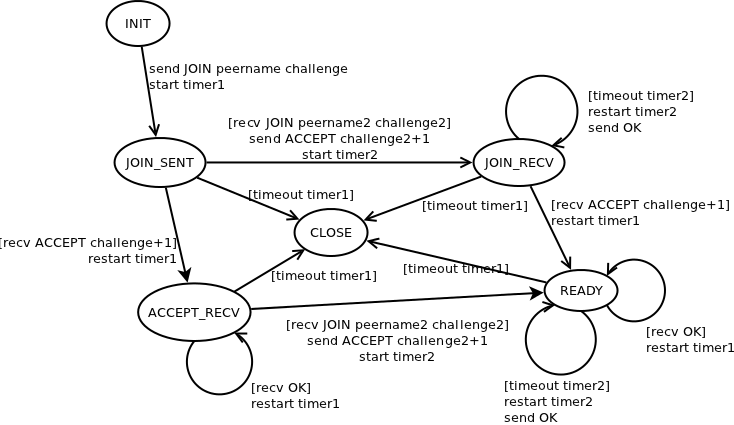
\includegraphics[width=0.9\textwidth]{peerhandler}
  \caption{Diagramme d'états illustrant le comportement d'un pair
    contactant un autre pair ou d'un pair ayant été contacté par un autre
    pair}
  \label{fig:peerhandler}
\end{figure}

\subsection{Envoi du presse-papier}
Le presse-papier est envoyé lorsqu'un client local notifie le client
P2P qu'un copier a été effectué. Afin de permettre 

\subsection{Client local}
Le client P2P est le \emph{front-end} avec le réseau, il est chargé
de communiquer avec les pairs du réseau afin de les découvrir et savoir
lequel détient le presse-papier. Le front-end avec l'utilisateur
est en revanche le client local. Celui-ci tourne sur le même ordinateur
que le client P2P, se charge d'envoyer le contenu du presse-papier
lors d'une copie de l'utilisateur, et lui demande le contenu du presse-papier
lorsque que l'utilisateur effectue un coller.
De même le client P2P envoie le contenu du presse-papier au client local si
ce dernier a envoyé une requête pour l'obtenir ou si un autre ou un autre
client local a changé le contenu du presse-papier.

Cependant, contrairement au client P2P, il peut y avoir plusieurs clients
locaux tournant sur le même ordinateur. Chacun d'entre eux étant destiné
à un environnement précis. Dans ce projet, seront développés deux types
de clients différents:
\begin{itemize}
\item Un client tournant en tâche de fond (comme \emph{daemon}) et
  synchronisant le contenu du presse-papier de X Window.
\item Un client gérant le copier/coller dans un terminal, composé de deux
  logiciels:
  \begin{itemize}
  \item Une commande permettant de copier une donnée à partir de l'entrée
    standard du shell.
  \item Une commande permettant de coller une donnée sur la sortie standard
    du shell.
  \end{itemize}
\end{itemize}

\section{Protocoles}
Trois protocoles sont à définir afin de faire fonctionner l'application
correctement. Le premier est celui permettant de découvrir des pairs grâce au
broadcast. Le second est celui utilisé sur le réseau par les clients
P2P afin de communiquer entre eux. Le dernier est utilisé entre le client
P2P et les clients locaux afin de se notifier mutuellement de changements
dans le presse papier. De même ils doivent prendre en compte
l'aspect sécurité, en proposant un moyen d'identification.
Ces trois protocoles seront appelés respectivement protocole broadcast,
protocole P2P et protocole local.

Les protocoles sont caractérisés par un ensemble de types de messages.
Ceux-ci sont décrits en utilisant la syntaxe suivant:
\begin{verbatim}
MSG <SP> <VAR1> <SP> <VAR2> ... <SP> <VARN> <CRLF>
\end{verbatim}
MSG définit le type du message. Celui-ci contient $N$ variables
<VAR1>, <VAR2>, $\ldots$, <VARN>. Chacune est séparée par un espace (<SP>)
et le message se termine par un retour chariot (<CRLF>). Chaque variable est
ensuite décrite et le type de messages pouvant être reçu comme réponse est
décrit.

\subsection{Protocole broadcast}
\subsubsection*{JOIN}
Un message de type JOIN sert à authentifier un pair.
\begin{verbatim}
JOIN <SP> <NAME> <SP> <GROUP> <CRLF>
\end{verbatim}
\begin{description}
\item[Variable NAME:] identifiant du pair envoyant le message.
\item[Variable GROUP:] nom du groupe de pairs.
\item[Réponse:] si le pair n'est pas déjà présent dans la table des pairs,
  il faut ouvrir une connexion TCP avec celui-ci en utilisant le protocole P2P.
\end{description}

\subsection{Protocole P2P}
\subsubsection*{JOIN}
Un message de type JOIN sert à authentifier un pair.
\begin{verbatim}
JOIN <SP> <NAME> <SP> <CHALLENGE> <CRLF>
\end{verbatim}
\begin{description}
\item[Variable NAME:] identifiant du pair envoyant le message.
\item[Variable CHALLENGE:] un nombre généré aléatoirement utilisé comme
  challenge.
\item[Réponse:] un message ACCEPT où le challenge est incrémenté de un.
\end{description}

\hrulefill

\subsubsection*{ACCEPT}
Un message de type ACCEPT sert de réponse à un message JOIN.
\begin{verbatim}
ACCEPT <SP> <CHALLENGE> <CRLF>
\end{verbatim}
\begin{description}
\item[Variable CHALLENGE:] le challenge reçu dans le message JOIN
\item[Réponse:] Si le challenge ne correspond pas (\emph{i.e.} n'a pas été
  incrémenté de un et l'authentification a échoué), alors un KO est envoyé
  pour fermer la connexion.
\end{description}

\hrulefill

\subsubsection*{KO}
Ce type de message permet de signaler un refus ou une erreur et de fermer
la connexion.
\begin{verbatim}
KO <SP> <ERRNO> <CRLF>
\end{verbatim}
\begin{description}
\item[Variable ERRNO:] code d'erreur pouvant être:
  \begin{description}
  \item[0] fermeture de la connexion.
  \item[1] fermeture due à un timeout.
  \item[2] message ACCEPT non valide, échec de l'authentification.
  \item[3] type de données du message DATA inconnu. Pas de fermeture de la
    session, le contenu du presse-papier est simplement ignoré par le pair.
  \end{description}
\end{description}

\hrulefill

\subsubsection*{OK}
Ce type de message est envoyé à interval régulier afin de servir de mécanisme
de keep alive.
\begin{verbatim}
OK <CRLF>
\end{verbatim}

\hrulefill

\subsubsection*{DATA}
Un message de type DATA permet d'envoyer le contenu du presse-papier.
Le contenu presse-papier peut être fragmenté et être envoyé dans plusieurs
messages DATA. Ceci permet d'éviter d'avoir à envoyer un message DATA très
long dans le cas d'un presse-papier de grande taille et ainsi d'être sûr
que les keep alive OK seront biens transmis.
\begin{verbatim}
DATA <SP> <TYPE> <SP> <MORE> <SP> <LENGTH> <SP> <CONTENT> <CRLF>
\end{verbatim}
\begin{description}
\item[Variable TYPE:] cette variable permet de préciser le type
  de donnée et ainsi d'étendre facilement le protocole afin de supporter
  d'autres types de données. Dans ce cas il faudra préciser comment ce type
  de données est encodé.
  \begin{description}
  \item[0] texte.
  \end{description}
\item[Variable MORE:] vaut 1 s'il y a encore des données fragmentées qui
  suivent, 0 sinon.
  Si la variable vaut 1, alors il faut bufferiser le contenu du message
  jusqu'à ce qu'à recevoir un message DATA avec cette variable égale à 0.
\item[Variable LENGTH:] longueur de la donnée en bytes.
\item[Variable CONTENT:] contenu de la donnée dont la longueur
  doit vérifier la variable LENGTH.
\end{description}

\subsection{Protocole local}
\subsubsection*{GET}
Ce type de message est envoyé par le client local pour demander au client P2P
d'envoyer le contenu du presse-papier.
\begin{verbatim}
GET <CRLF>
\end{verbatim}

\hrulefill

\subsubsection*{DATA}
Un message de type DATA permet d'envoyer le contenu du presse-papier. Un tel
message peut aussi bien être envoyé par le client P2P que par le client local.
\begin{verbatim}
DATA <SP> <TYPE> <SP> <LENGTH> <SP> <CONTENT> <CRLF>
\end{verbatim}
\begin{description}
\item[Variable TYPE:] cette variable permet de préciser le type
  de donnée et ainsi d'étendre facilement le protocole afin de supporter
  d'autres types de données. Dans ce cas il faudra préciser comment ce type
  de données est encodé.
  \begin{description}
  \item[0] texte.
  \end{description}
\item[Variable LENGTH:] longueur de la donnée en bytes.
\item[Variable CONTENT:] contenu de la donnée dont la longueur
  doit vérifier la variable LENGTH.
\end{description}
